\section{Auswertung}
\label{sec:Auswertung}

\subsection{Temperaturverläufe}
Die gemessenen Temperaturen $T_1$ und $T_2$, sowie die Drücke
$p_a$ und $p_b$ und die Leistungsaufnahme des Kompressors
zu verschiedenen Zeiten $t$ sind in Tabelle \ref{tab1}
dargestellt.
\newline
Die Temperaturverläufe der beiden Reservoire sind in Abbildung
\ref{fig:plot1} zu sehen.
%\begin{table}\caption{Der maximale Drehimpuls $L$, der Gesamtspin $S$ und der Gesamtdrehimpuls $J$ ergeben sich zum Landé-Faktor $g_\text{J}$ für die vier verschiedenen Elemente.}
\label{tab1}
\centering
\sisetup{round-mode = places, round-precision=2, round-integer-to-decimal=true}
\begin{tabular}{S[]S[]S[]S[]} 
\toprule
{$L$} & {$S$} & {$J$} & {$g_\text{J}$}\\
\midrule
5.0 & 1.0 & 4.0 & 0.8\\
0.0 & 3.5 & 3.5 & 2.0\\
6.0 & 1.5 & 4.5 & 0.7272727272727273\\
5.0 & 2.5 & 7.5 & 1.3333333333333333\\
\bottomrule
\end{tabular}\end{table}

\begin{figure}
    \centering
    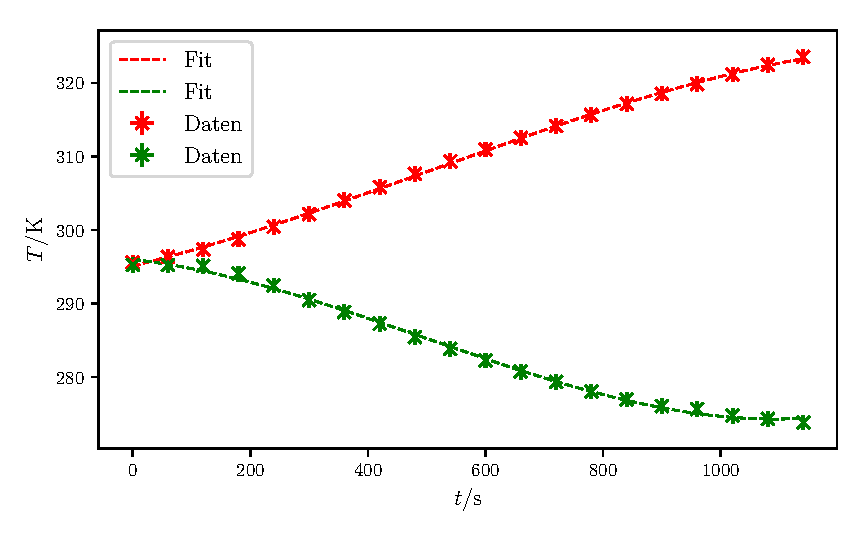
\includegraphics[width=10cm, height=10cm]{build/plot1.pdf}
    \caption{Temperaturverläufe. Es sind jeweils die Daten und ein Fit dargestellt.
    Die rote Kurve stellt ... dar. Die grüne Kurve stellt ... dar.
    % Die Fitparameter der Kurve der Temperatur im ersten Reservoir sind $A=\num{(-1.20 \pm 17.01)e-8}$,
    % $B=\num{(1.83 \pm 29.53)e-5}$, $C=\num{(1.95 \pm 14.27)e-2}$ und $D=\SI{295.11 \pm 0.18}$.
    % Die Fitparameter der Kurve der Temperatur im zweiten Reservoir sind $A=\num{}$,
    % $B=\num{}$, $C=\num{}$ und $D=\num{}$.
    }
    \label{fig:plot1}
\end{figure}

Die Differentialquotienten $\frac{dT}{dt}$ für vier verschiedene Temperaturen
sind im Folgenden zu sehen. Es werden die Temperaturen
\begin{align*}
    T_1 &= \SI{1}{\degreeCelsius} &= \SI{274.15}{\kelvin} \\
    T_2 &= \SI{5}{\degreeCelsius} &= \SI{278.15}{\kelvin}\\
    T_3 &= \num{10}{\degreeCelsius} &= \SI{283.15}{\kelvin}\\
    T_4 &= \num{15}{\degreeCelsius} &= \SI{288.15}{\kelvin}
\end{align*}
Für $\frac{dT_1}{dt}$:
\begin{align*}
    dT_{1,1} &= \num{} \\
    dT_{1,2} &= \num{} \\
    dT_{1,3} &= \num{} \\
    dT_{1,4} &= \num{}
\end{align*}
Für $\frac{dT_2}{dt}$:
\begin{align*}
    dT_{2,1} &= \num{} \\
    dT_{2,2} &= \num{} \\
    dT_{2,3} &= \num{} \\
    dT_{2,4} &= \num{}
\end{align*}

\subsection{Bestimmung der Güteziffer}
Die realen Güteziffern für die vier Temperaturen werden mittels
Gleichung \eqref{eqn:} %Gleichung
berechnet.
Die idealen Güteziffern werden mit Gleichung \eqref{eqn:} %Gleichung
bestimmt.
Beide Größen sind in Tabelle \ref{tabsolution1} jeweils
gegenübergestellt.
\begin{table}
\caption{Die Ergebnisse für die realen und idealen Gütewerte für die vier verschiedenen Temperaturwerte.}
\label{tabsolution1}
\centering
\begin{tabular}{S[table-format=1.2]  
        @{${} \pm{}$}
        S[table-format=1.2]
        @{$  $}
        S[table-format=5.1]
        @{${} \pm{}$}
    S[table-format=3.1]}
\toprule
   \multicolumn{2}{c}{$\nu_\text{real}$} &\multicolumn{2}{c}{$\nu_\text{ideal}$}\\
\midrule
    0.64 & 0.05 & 270.0 & 350.0\\
    0.67 & 0.06 & 25.8 & 3.1\\
    0.68 & 0.1 & 10.8 & 0.5\\
    0.54 & 0.16 & 7.5 & 0.23\\
\bottomrule
\end{tabular}\end{table}


\subsection{Bestimmung des Massendurchsatzes}
Das im Versuch verwendete Gas ist Dichlordifluormethan.
Die Verdampfungswärme $L$ des Gases wird durch die Dampfdruck-Kurve
in Abb. \ref{fig:plot2} bestimmt. %wie?
Die Wertepaare des Drucks $p$ und der Temperatur $T$, die zur
Darstellung der Dampfdruck-Kurve nötig sind, befinden sich in
Tabelle \ref{tab2}. 
\begin{table}\caption{Das Verhältnis des magnetischen Feldes durch die Beschleunigungsspannung aufgetragen gegen die Höhe.}
\label{tab2}
\centering
\sisetup{round-mode = places, round-precision=2, round-integer-to-decimal=true}
\begin{tabular}{S[]S[]S[]} 
\toprule
{$B_1 / \si{\henry}$} & {$B_2 / \si{\henry}$} & {$\frac{D}{(L^2 + D^2)} / \si{\per\meter}$}\\
\midrule
0.0 & 0.0 & 0.0\\
3.5649278338607584e-07 & 3.862005153349155e-07 & 0.29289724188430566\\
8.912319584651897e-07 & 8.912319584651897e-07 & 0.5827222842713544\\
1.4259711335443034e-06 & 1.396263401595464e-06 & 0.8665094112549946\\
1.9250610302848096e-06 & 1.8418793808280586e-06 & 1.1414982164090373\\
2.3885016486867084e-06 & 2.3172030920094934e-06 & 1.4052180429996723\\
2.923240823765822e-06 & 2.822234535139767e-06 & 1.6555530006898145\\
3.4223307205063282e-06 & 3.3272659782700412e-06 & 1.8907846756403912\\
\bottomrule
\end{tabular}\end{table}
\begin{figure}
    \centering
    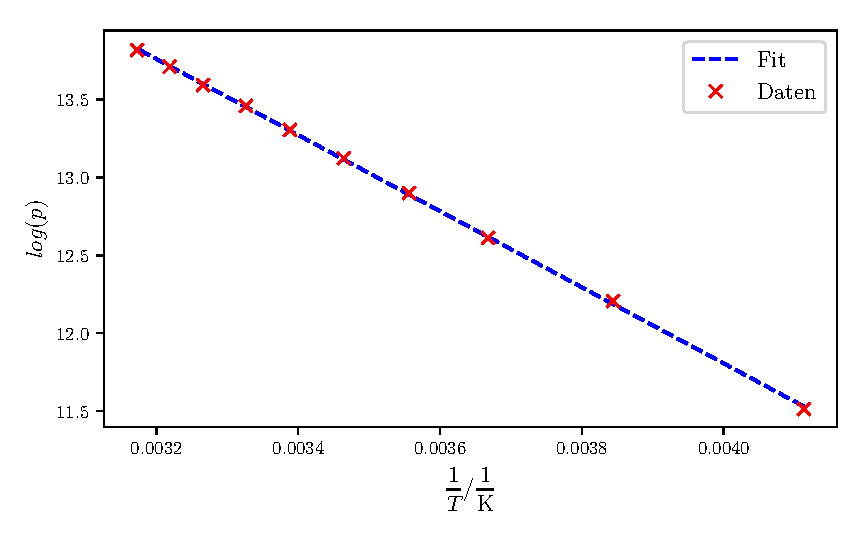
\includegraphics[width=10cm, height=10cm]{build/plot2.pdf}
    \caption{Plot2}
    \label{fig:plot2}
\end{figure}
\begin{equation*}
    L = \SI{}{} %Verdampfungswärme
\end{equation*}
\begin{align*}
    m_1 &= \SI{}{} \\
    m_2 &= \SI{}{} \\
    m_3 &= \SI{}{} \\
    m_4 &= \SI{}{}
\end{align*}

\subsection{Bestimmung der mechanischen Kompressorleistung}
Dichlordifluormethan hat bei den Werten
\begin{align*}
    T &= \SI{273.15}{\kelvin} \\
    p &= \SI{e5}{\pascal} \\
    \kappa &= \num{1.14}
\end{align*}
die Dichte 
\begin{equation*}
    \rho_0 = \SI{5.51}{\gram\per\liter}.
\end{equation*}
Die mechanischen Kompressorleistungen für die vier Temperaturen
ergeben sich mit Gleichung \eqref{eqn:} %Gleichung
zu den in Tabelle \ref{tabsolution2} stehen Werten.
\begin{table}\caption{Die Ergebnisse für die mechanische und die elektrische Leistung für die vier verschiedenen Temperaturwerte.}
\label{tabsolution2}
\centering
\sisetup{round-mode = places, round-precision=2, round-integer-to-decimal=true}
\begin{tabular}{S[]S[]} 
\toprule
{\nu_\text{real}} & {\nu_\text{ideal}}\\
\midrule
 135 \pm 32 & 165\\
 160 \pm 40 &  200\\
 50 \pm 70 & 208\\
 310 \pm 140 & 212\\
\bottomrule
\end{tabular}\end{table}
